\documentclass[letterpaper, 12pt]{report}

\usepackage[utf8]{inputenc}
\usepackage[english, spanish]{babel}
\usepackage{fullpage} % changes the margin
\usepackage{graphicx}
\usepackage{amsmath}
\usepackage{enumitem}
\usepackage{chngcntr}
\usepackage{setspace}
\usepackage{url}
\usepackage{csquotes}
\usepackage{float}
\usepackage{verbatim}
\usepackage{tabularx}
\usepackage{amsmath}

\counterwithin{figure}{section}
\renewcommand{\thesection}{\arabic{section}}
\renewcommand{\thesubsection}{\thesection.\arabic{subsection}}
\renewcommand{\baselinestretch}{1.5}

\usepackage[style=numeric, maxnames=6, minnames=3, backend=biber, parentracker=true, sorting=none]{biblatex}
\DefineBibliographyStrings{english}{%chktex-file 1 chktex-file 6
      andothers = {\em et\addabbrvspace al\adddot}
}
\addbibresource{./Bibliography/bibliography.bib}

\usepackage{array}
\usepackage{enumitem}

\usepackage{setspace}
\setlength{\parskip}{\baselineskip}

\begin{document}

\section*{Experimento 1}

\begin{itemize}[label=$\bullet$]
      \item \textbf{¿Por qué se desvía la aguja del galvanómetro cuando el imán entra o sale de la bobina?}

            Esto se debe a que al introducir el imán en el interior del
            solenoide se crea una corriente eléctrica (corrientes
            inducidas) que alimenta a la bobina y produce un campo
            magnético en la bobina, y cuando el imán entra y sale se
            genera una variación en ese campo magnético, por esta razón
            la aguja del galvanómetro se mueve.\@(principio de Oersted
            y Faraday)

      \item \textbf{¿Por qué la aguja se queda quieta cuando el imán permanece en reposo dentro de la
                  bobina?}
            Siguiendo la lógica anterior, para que haya corriente eléctrica en la bobina, debe haber
            movimiento en el campo magnético, es decir, cuando el imán se queda en reposo
            dentro de la bobina la inducción de corriente eléctrica es nula, por lo tanto, si no hay
            movimiento en el imán o en la bobina, el campo magnético permanece constante, por
            eso la aguja no se mueve.

      \item \textbf{Hacia dónde se desvió la aguja del galvanómetro cuando el
                  imán entró a la bobina?}

            Debido a la interacción de los campos magnéticos, la aguja
            del galvanómetro se desvía dependiendo de la polaridad del
            imán y de la dirección de la corriente inducida en la
            bobina. En este caso se desvía hacia la derecha.

      \item \textbf{¿Hacia dónde se desvió la aguja del galvanómetro cuando el imán
                  salió de la bobina?}

            Basándose en la lógica anterior, la dirección de la
            desviación de la aguja del galvanómetro será opuesta a
            cuando ingreso, es decir, se desvía hacia la izquierda

      \item \textbf{Dibuje un esquema donde se indique la dirección de la
                  corriente inducida en una de las espiras de la bobina y la
                  polaridad que debió tener el campo magnético (norte o sur)
                  cuando el imán entra. Sugerencia: Utilice la ley de Lenz
                  para su razonamiento.}

            \begin{figure}[H]
                  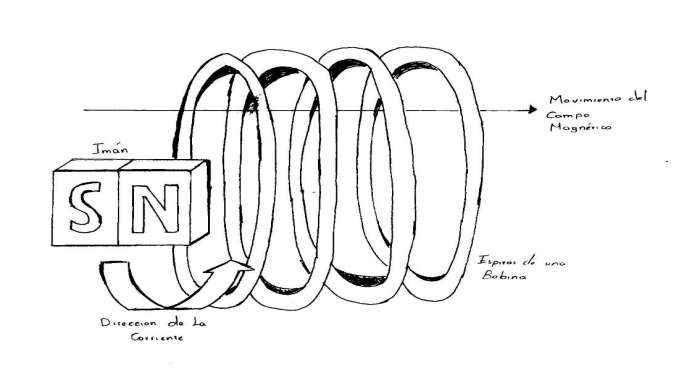
\includegraphics[width=0.9\linewidth]{./Images/ImagenBobina.png}
            \end{figure}

      \item \textbf{¿Cuál es la polaridad del extremo A y del extremo B del imán? Utilice una brújula y
                  verifique si su respuesta es correcta (ver figura 2).}

            El extremo A (rojo) es el polo sur y el extremo B (verde) es el polo norte.
\end{itemize}

\section*{Experimento 2}

\begin{itemize}[label=$\bullet$]
      \item \textbf{Observe que en el transformador las bobinas se mantienen
                  unidas por un núcleo de hierro, pero éste no realiza
                  ninguna conexión eléctrica entre las bobinas. ¿Por qué se
                  mueve la aguja del galvanómetro solamente en el instante en
                  que se abre y se cierra el interruptor?}

            Esto sucede porque al abrir el interruptor la corriente
            eléctrica de la fem comienza a fluir por la bobina
            primaria, lo cual, genera un campo magnético el cual induce
            una corriente eléctrica en la bobina secundaria cuyos
            extremos están conectados al galvanómetro, posteriormente
            el galvanómetro detecta una corriente eléctrica y por ende
            se mueve la aguja. Luego se cierra el interruptor y la
            corriente deja de fluir por la bobina primaria, esto
            implica que el campo magnético también varíe haciendo que
            el galvanómetro vuelva a detectar una corriente eléctrica
            provocando un movimiento en su aguja.

      \item \textbf{Cuando el interruptor permanece cerrado, ¿por qué no se
                  desvía la aguja del galvanómetro?}

            Al estar el interruptor cerrado no hay corriente eléctrica
            fluyendo por la bobina primaria, lo cual, hace imposible la
            generación de un campo magnético, y si no hay corriente
            fluyendo hacia la bobina secundaria el galvanómetro no
            detectara nada, por ende, la aguja no se mueve.
\end{itemize}

\section*{Experimento 3}

\begin{itemize}[label=$\bullet$]
      \item \textbf{¿Qué es una fuente de corriente alterna?}

            Es un tipo de corriente que cambia de dirección y magnitud
            de forma periódica, es decir, produce una corriente
            eléctrica que fluye primero en una dirección y luego en la
            dirección opuesta, a intervalos regulares de tiempo.

      \item \textbf{¿Por qué no oscila la indicación del voltímetro si la alimentación y salida es de
                  corriente alterna?}

            Aunque es innegable la oscilación presente en las
            corrientes alternas los voltímetros utilizados en la
            medición de corriente alterna están diseñados para medir y
            mostrar un valor constante o absoluto del voltaje, el cual,
            oscila entre un valor positivo y un valor negativo.

      \item \textbf{¿Por qué ahora cuando el interruptor permanece cerrado siempre el voltímetro está
                  indicando un voltaje?}

            Cuando el interruptor permanece cerrado, se establece una
            conexión eléctrica continua entre la fuente de voltaje y el
            circuito eléctrico, lo que significa que hay un flujo
            constante de corriente eléctrica a través del circuito.
            Ahora bien, al momento de medir el voltaje con el
            voltímetro se visualiza una diferencia considerable debido
            a la pérdida del flujo magnético (el núcleo de hierro esta
            abierto).

      \item \textbf{¿Cuándo se retira la parte superior del núcleo, por qué disminuye la amplitud del
                  voltaje inducido en la bobina secundaria?}

            La cantidad de voltaje inducido en la bobina secundaria de
            un transformador está directamente relacionada con el
            numero de vueltas o espiras y la diferencia de flujo
            magnético que atraviesa la bobina secundaria. Como el
            núcleo de hierro esta abierto el flujo magnético se esta
            perdiendo en gran cantidad

      \item \textbf{¿Por qué la amplitud del voltaje inducido disminuye cuando la bobina primaria tiene
                  más vueltas que la secundaria?}

            Por el principio de los transformadores que dice que la
            cantidad de tensión es directamente proporcional al número
            de vueltas que posee la bobina.

      \item \textbf{¿Cuál es la función principal de un transformador?}

            Un transformador es un dispositivo que utiliza la inducción
            electromagnética para transferir energía eléctrica de un
            circuito a otro mediante la variación del voltaje y la
            corriente en los circuitos, por lo que su función principal
            es aumentar o disminuir el voltaje y la corriente de la
            energía eléctrica, lo que permite que la energía se
            transmita más eficientemente a través de largas distancias
            y se adapte a las necesidades de diferentes tipos de
            equipos.
\end{itemize}

\section*{Experimento 4}

\begin{itemize}
      \item \textbf{El esquema es el equivalente al montaje experimental de la
            práctica, por lo que ya esta incluido en el informe.}

      \item \textbf{¿De qué depende el impulso con que sale despedido el anillo sin ranura?}

            La fuerza de repulsión depende de varios factores,
            incluyendo la corriente, el voltaje suministrado, las
            vueltas de la bobina o incluso las propiedades de los
            materiales de los anillos.

      \item \textbf{¿Por qué se produce una chispa cuando se unen los extremos del cable?}

            El punto superior $(V_a)$ y el punto inferior $(V_b)$ están a
            diferente potencial, por lo que al juntar los extremos del
            cable se produce una chispa.

      \item \textbf{¿Por qué se enciende el bombillo si no tiene ninguna fuente conectada? ¿Por qué
            aumenta la luminosidad a medida que se introduce más en el tubo?}

            Debido al campo magnético, básicamente por el fenómeno de
            Inducción electromagnética, en el cual se puede inducir
            corriente por medio de un campo magnético. En ese sentido a
            medida que el bombillo se va introduciendo más en el tubo,
            va sintiendo un campo magnético mayor, por lo que la
            corriente inducida también lo será.

      \item \textbf{Si el aluminio no tiene propiedades magnéticas, ¿Por qué
            levita, y hasta expulsado, el cilindro sin ranura?}

            El aluminio no se siente atraído por un imán debido a que
            el orden de las moléculas no forma un campo con gran
            dominio magnético. Un dominio magnético corresponde a una
            región que se encuentra dentro de un material en el cual
            sus átomos se organizan de tal forma que crean un campo
            magnético uniforme, ya que los momentos magnéticos de cada
            átomo se alinean con el otro apuntando hacia una misma
            dirección formando un dipolo. Además, cabe mencionar que el
            aluminio no se siente atraído por los imanes debido a que
            no tiene propiedades magnéticas permanentes. A pesar de
            esto, el aluminio junto con otros metales son los mejores
            materiales conductores de electricidad. Entonces, al ser de
            aluminio el cilindro, un material conductor, al moverse a
            través del campo magnético de la bobina, se genera una
            corriente eléctrica en su interior, lo que produce un campo
            magnético que se opone al original y produce la fuerza de
            levitación.

      \item \textbf{¿Por qué el cilindro con ranura no levita?}

            Se debe a que el objeto no debe tener ninguna ranura para
            poder levitar debido a que ese tipo de imperfecciones
            impiden el flujo de corriente eléctrica (se ven
            interrumpidas en la grieta o ranura), lo que imposibilita
            la creación del campo magnético.
\end{itemize}

\newpage

\printbibliography

\end{document}